% Created 2021-03-19 Fri 00:52
% Intended LaTeX compiler: pdflatex
\documentclass[letterpaper, 11pt]{article}
\usepackage{lmodern} % Ensures we have the right font
\usepackage[T1]{fontenc}
\usepackage[utf8]{inputenc}
\usepackage{graphicx}
\usepackage{amsmath, amsthm, amssymb}
\usepackage[table, xcdraw]{xcolor}
\renewcommand*{\contentsname}{Conteúdo}
\renewcommand*{\listfigurename}{Lista de figuras}
\usepackage{titling}
\setlength{\droptitle}{-6em}
\setlength{\parindent}{0pt}
\setlength{\parskip}{1em}
\usepackage[stretch=10]{microtype}
\usepackage{hyphenat}
\usepackage{ragged2e}
\usepackage{subfig} % Subfigures (not needed in Org I think)
\usepackage{hyperref} % Links
\usepackage{listings} % Code highlighting
\usepackage[top=1in, bottom=1.25in, left=1.55in, right=1.55in]{geometry}
\renewcommand{\baselinestretch}{1.15}
\usepackage[explicit]{titlesec}
\pretitle{\begin{center}\fontsize{20pt}{20pt}\selectfont\Huge\bfseries}
\posttitle{\par\end{center}}
\preauthor{\begin{center}\vspace{-6bp}\fontsize{14pt}{14pt}\selectfont}
\postauthor{\par\end{center}\vspace{-25bp}}
\predate{\begin{center}\fontsize{12pt}{12pt}\selectfont}
\postdate{\par\end{center}\vspace{0em}}
\titlespacing\section{0pt}{10pt}{10pt} % left margin, space before section header, space after section header
\titlespacing\subsection{0pt}{10pt}{10pt} % left margin, space before subsection header, space after subsection header
\titlespacing\subsubsection{0pt}{10pt}{10pt} % left margin, space before subsection header, space after subsection header
\usepackage{enumitem}
\setlist{itemsep=-2pt} % or \setlist{noitemsep} to leave space around whole list
\author{Bruno Alexandre Ferreira Pinto Teixeira (a2019100036)}
\date{\ldots{}}
\title{Relatório \ldots{}\\\medskip
\large Departamento de Engenharia Informática e de Sistemas (DEIS)}
\hypersetup{
 pdfauthor={Bruno Alexandre Ferreira Pinto Teixeira (a2019100036)},
 pdftitle={Relatório \ldots{}},
 pdfkeywords={},
 pdfsubject={},
 pdfcreator={Emacs 26.3 (Org mode 9.1.9)}, 
 pdflang={English}}
\begin{document}

\maketitle
;; \url{https://www.fbxiang.com/blog/2017/11/01/write\_papers\_with\_org\_mode\_and\_spacemacs.html}

\begin{center}

\includegraphics[width=5 cm]{images/isec.png}
\end{center}

\clearpage
\tableofcontents
\clearpage

\listoffigures
\clearpage

\section{Introdução}
\label{sec:org16d332e}
\paragraph{}
Neste relatório apresentamos a arquitetura assim como o funcionamento do trabalho prático.\\
Durante as várias metas existiram algumas mudanças, no entanto todas as mudanças são descritas e apresentadas de forma a justificar o porquê dessas mudanças terem sido feitas.

\clearpage

\section{Desenvolvimento}
\label{sec:org99c3fd6}

\subsection{Arquitetura}
\label{sec:org3d5d926}

\paragraph{}
Para este trabalho usamos uma arquitetura cliente servidor, em que o servidor é designado por árbitro e o cliente é uma interface para um jogador.\\
Cada jogador usa um cliente(shell), cliente este que interage com um servidor, ou seja, existem múltiplos clientes mas só um servidor.\\
O servidor é responsável pela criação dos jogos, pelo redirecionamento entre jogos e clientes e pela manutenção de toda a estrutura do programa.
\paragraph{}
Na figura seguinte mostramos um exemplo da arquitetura, com todos os pormenores, em que existem dois clientes, um arbitro e um jogo para cada cliente.


\begin{figure}[htbp]
\centering
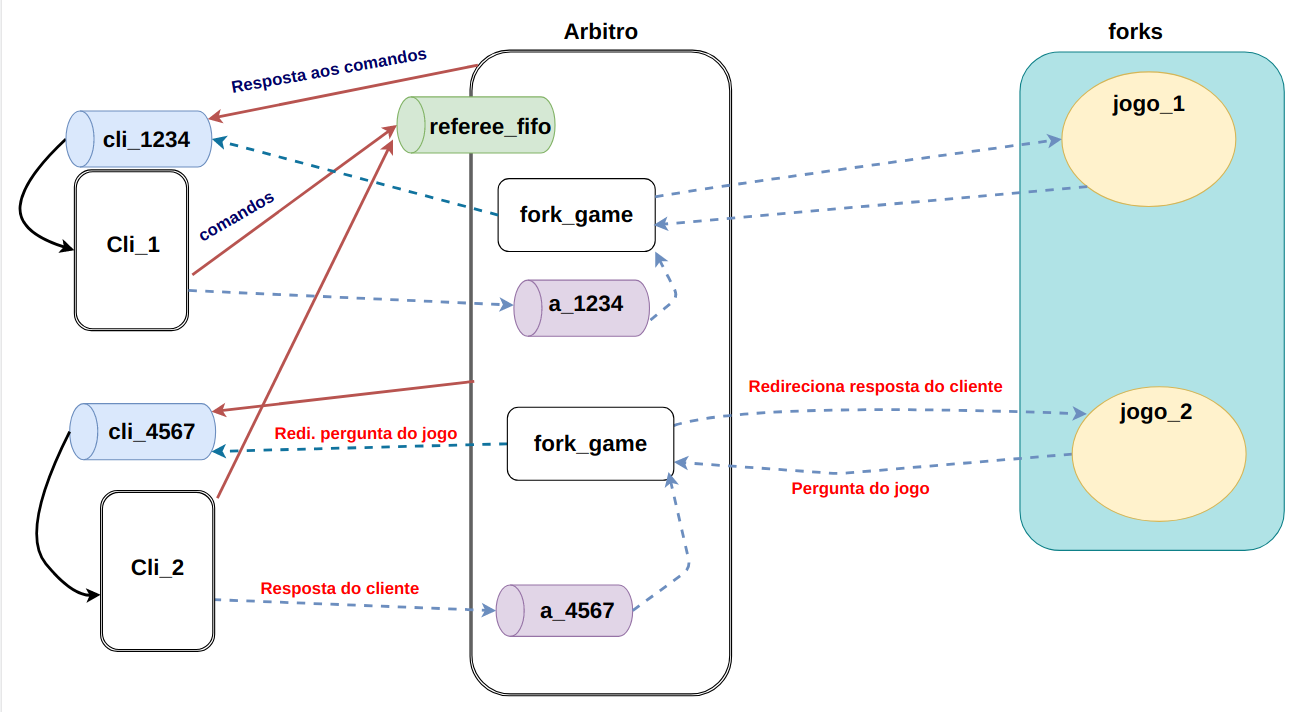
\includegraphics[width=.9\linewidth]{images/esquema.png}
\caption{\label{fig:org42eb751}
exemplo de caption de uma imagem}
\end{figure}


\subsubsection{Estruturas}
\label{sec:org8a0ba9d}

\paragraph{}
Consoante a realização do trabalho, decidimos fazer algumas alterações a algumas estruturas assim como acrescentar outras.
\paragraph{}
À estrutura \textbf{Games} foi-lhe retirado um campo, \textbf{pergunta}, pois não era utilizado.\\
A estrutura \textbf{Player} manteve-se, apenas foi adicionado o \textbf{player\_trinco} sendo este um \textbf{mutex} para trabalhar com os respetivos dados e continua a ser usada para identificar um jogador num array dinâmico de estruturas.\\

Foi tambem criada uma nova estrutura, \textbf{Mainframe}, que é usada para a passagem de informação para as threads. Esta estrutura contém tanto o array de jogadores como o array de jogos existentes, o tempo de espera (wait time) e o tempo do campeonato,assim como algumas flags. \\
A estrutura \textbf{User}, presente tanto no \textbf{referee} como no \textbf{client}, manteve-se igual à meta anterior.

\subsubsection{Threads}
\label{sec:org44f4fa0}

\paragraph{}
Foram desenvolvidas três funções thread além da main thread.
\paragraph{}
Temos a \textbf{thread\_register}, função usada para fazer a leitura do \textbf{pipe do arbitro} e proceder consoante a leitura, quer adicionar um novo jogador quer ler um comando do cliente. Esta thread é responsável também por lançar a \textbf{thread\_timer} quando tem 2 jogadores já inscritos.
\paragraph{}
A função \textbf{thread\_timer} cronometra o tempo de espera, antes de lançar um campeonato, e antes de cronometrar o tempo de duração do mesmo, escolhe de forma aleatória o jogo.\\

Esta thread lança uma thread chamada de \textbf{fork\_game} para cada \textbf{jogador}.\\
A \textbf{thread\_timer} notifica os jogadores sobre o inicio, o fim e o respetivo score do campeonato.
\paragraph{}
A thread \textbf{fork\_game} é responsavel por realizar o \textbf{fork dos jogos} bem como executar o jogo(usando o \textbf{execl}). Nesta thread fazemos todo o processo de \textbf{reencaminhamento} entre o \textbf{cliente} e o seu respetivo \textbf{jogo}.
\paragraph{}
Após o fim do tempo do campeonato e do encerramento de todas as threads é recomeçado outro campeonato. 

\subsection{Funcionamento}
\label{sec:org160e711}

\paragraph{}
O arbitro é iniciado e fica à espera de pelo menos dois jogadores para conseguir iniciar um campeonato.\\
Quando dois clientes são iniciados, é feita uma verificação caso o nome dos mesmos seja igual uma vez que não faz sentido terem ambos o mesmo nome.\\
Depois de todas as validações feitas, esses clientes são colocados num campeonato, campeonato este que é totalmente administrado pelo árbitro.\\
O campeonato consiste num jogo simples em que ganha quem tiver melhor pontuação no final do tempo.\\
Dentro deste processo existem várias comunicações internas que precisam de ser esclarecidas para que seja mais fácil entener o funcionamento do trabalho.
\paragraph{}
O cliente gere um \textbf{FIFO}, \textbf{FIFO} este que vai receber algumas informações sempre que se quiser comunicar com o cliente.\\
O arbitro também tem um \textbf{FIFO} próprio que é usado para receber comandos vindos do cliente, comandos pessoais, não relativos aos jogos.
\paragraph{}
Quando um jogador é inscrito, é criado um \textbf{FIFO} designado por (a\_PID\_DO\_JOGADOR) que é usado unica e exclusivamente para a comunicação entre cliente e jogo, sendo este processo de comunicação, um processo indireto.\\
Quando o campeonato começa, o arbitro lança algumas threads (explicadas anteriormente), sendo uma delas responsável pela comunicação entre jogo e cliente. Neste processo de comunicação, o jogo envia uma mensagem para a thread \textbf{fork\_game} e a thread reencaminha a mensagem para o \textbf{FIFO} do cliente. Quando o cliente responde, é enviada uma mensagem para o \textbf{FIFO} (a\_PID\_DO\_JOGADOR), a thread (\textbf{fork\_game}) lê desse \textbf{FIFO} e redireciona a mensagem de volta para o jogo.
\paragraph{}
A inscrição e a saida de um jogador num campeonato só pode ser feita durante o tempo de espera entre campeonatos, ou seja, enquanto o campeonato não está a decorrer o jogador pode sair de maneira correta.
\paragraph{}
Quando o campeonato termina, os jogos são apagados enviando um sinal para cada jogo, as threads são terminadas e é recolhida a informação da pontuação de todos os jogadores, mostrando a todos os jogadores a sua pontuação e a melhor daquele campeonato.Quando o arbitro termina, todos os \textbf{FIFOS} são fechados e eliminados.

\section{Conclusão}
\label{sec:org130fa96}

\paragraph{}
Após a realização do trabalho, não foi encontrado nenhum \textbf{bug} que pusesse em causa a execução e a comunicação do \textbf{arbitro} e do \textbf{cliente}.\\
Foram testados vários cenários para que não houvesse problemas antes, durante e após a execução do \textbf{arbitro} e do \textbf{cliente}.
\paragraph{}
Uma vez que é usada memória dinâmica em vários pontos do trabalho, foi dada uma atenção extra para que não haja um \textbf{memory leak}.\\
No recomeço do campeonato verificamos tambem (com ajuda do \textbf{ps aux}) se todos os processos criados no campeonato anterior foram eliminados de maneira correta.
\paragraph{}
No final da execução do \textbf{arbitro} foi visto que todas as threads terminam de forma ordenada e correta e que todos os \textbf{FIFOS} são eliminados não deixando nenhum tipo de lixo no ambiente do utilizador.
\end{document}
